\documentclass[a4paper]{article}

\usepackage[french]{babel}
\usepackage[T1]{fontenc}
\usepackage[utf8]{inputenc}
\usepackage{amsmath}
\usepackage{graphicx}
\usepackage{lmodern}
\usepackage[left=3cm, right=3cm, bottom=4cm, top=4cm]{geometry}
\usepackage{array}
\usepackage{pdfpages}

\usepackage[gen]{eurosym}
\DeclareUnicodeCharacter{20AC}{\euro{}}

\usepackage{hyperref}

\title{
\textsc{Jeu SmallWorld\\
\LARGE Rapport de conception}
}

\author
{
	Hyuk-Chan {\sc Kwon}\\
    Florent {\sc Mallard}\\
}

\date{\today}

\begin{document}
\maketitle
\begin{center}
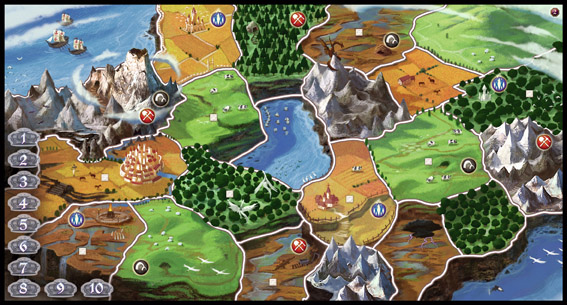
\includegraphics[width=0.8\textwidth]{./smallworld.jpg}~\\[5cm]
\end{center}

\newpage
\tableofcontents
\newpage


\section*{Introduction}
Le projet de Programmation et de Modélisation Orientées Objet se porte sur la réalisation d'un jeu inspiré de SmallWorld. Il s'agit d'un jeu de stratégie à deux joueurs dans lequel chacun dirige un peuple. Les unités des peuples bougent sur les cases de la carte afin de les conquérir, et combattent les unités ennemies. Le but est de contrôler plus de cases que son adversaire.\\
Nous allons aborder les thèmes principaux de la phase d'analyse et de conception.
Nous y expliquerons nos choix de conception  et de modélisation de notre jeu. Nous commencerons par effectuer un rappel des règles afin de distinguer les actions possibles.
Les étapes d'analyse ainsi que les différents diagrammes (classe, séquence, cas d'utilisation) figurent également dans ce rapport.
Nous expliquerons également notre utilisation des patrons de conception.

\section{Principes et But du jeu}
	\subsection{Règles du jeu}
		\subsubsection{Peuples}
Les joueurs ont le choix entre trois peuples : les Orcs, les Elfs et les Nains. Chacun dispose de bonus et malus influant sur la façon de les jouer.

\paragraph{Elfs} Les Elfs ont un coût de déplacement réduit de moitié sur une case Forêt, tandis que le déplacement sur une case Déserte est deux fois plus coûteux. Lors d'un combat dont l'issue conduit à la mort de l'unité, celle-ci a 50\% de chance de s'échapper avec 1 point de vie.
\paragraph{Orcs} Les Orcs ont un coût de déplacement 50\% sur une case Plaine. Ils ne gagnetn aucun point sur une case Forêt, mais ont un bonus propre à l'unité lorsque celle-ci en tue une autre.
\paragraph{Nains} Les Nains ont un coût de déplacement divisé par deux sur une case Plaine. Ils n'acquièrent aucun point sur les cases de ce type. Ils peuvent se déplacer d'une case Montagne à une autre à condition que celle-ci ne soit pas occupée par une unité adverse.

\subsubsection{Cartes}
Le joueur, à la création de la partie, a le choix entre trois cartes :
\begin{itemize}
\item Démo : 2 joueurs, 5 cases x 5 cases, 5 tours, 4 unités par peuple.
\item Petite : 2 joueurs, 10 cases x 10 cases, 20 tours, 6 unités par peuple.
\item Normale : 2 joueurs, 15 cases x 15 cases, 30 tours, 8 unités par peuple.
\end{itemize}

\subsubsection{Déroulement d'une partie}
Au début du jeu, chaque joueur choisit son peuple. Chaque peuple débute la partie avec toutes ses unités sur la même case de la carte, choisie de manière à ce que les joueurs ne soient pas trop proches. L’ordre de jeu est déterminé aléatoirement en début de partie. Les joueurs jouent chacun leur tour sur le même ordinateur.

\subsection{Tours de jeu}
Lorsqu’un joueur peut jouer (c.-à-d. une fois par tour), il peut déplacer toutes ses unités suivant leur nombre de points de déplacements (un déplacement sur une case coûte un point de déplacement). Il est possible pour chaque unité de passer son tour (généralement par le biais de la touche espace). Une unité combattante peut engager un combat s’il lui reste au moins un point de mouvement. Lorsqu’un joueur a fini son tour, il clique sur le bouton correspondant ("Fin tour"). C’est alors au joueur suivant de commencer son tour. La partie se termine lorsque le nombre de tours prédéfini en début de partie à été effectué, ou lorsqu’il ne reste qu’un seul joueur sur le plateau.

\section{Analyse}
\section{Fonctionnalités globales}
Après avoir lancé le jeu

\end{document}

